\section{Architecture}\label{sec:architecture}

\subsection{Context diagram (C4 Level 1)}\label{sec:context}

The context view sets the system's boundary. Everything the system knows about the
building comes through BuildSim's REST API. Everything it does to the building goes
back the same way. The operator uses a browser. The occupants are simulated inside
the system. I show them here as the people the system is for, because the safety
rules (interlocks) exist to protect them. There is one piece of outside compute, and
it is optional: the language model endpoint. When that detector is selected, the
service asks it about one room at a time. The other candidate was the overnight
model training from the proposal, and I did not need it. Nothing the system does to
the building depends on the endpoint answering.

\begin{figure}[H]
\centering
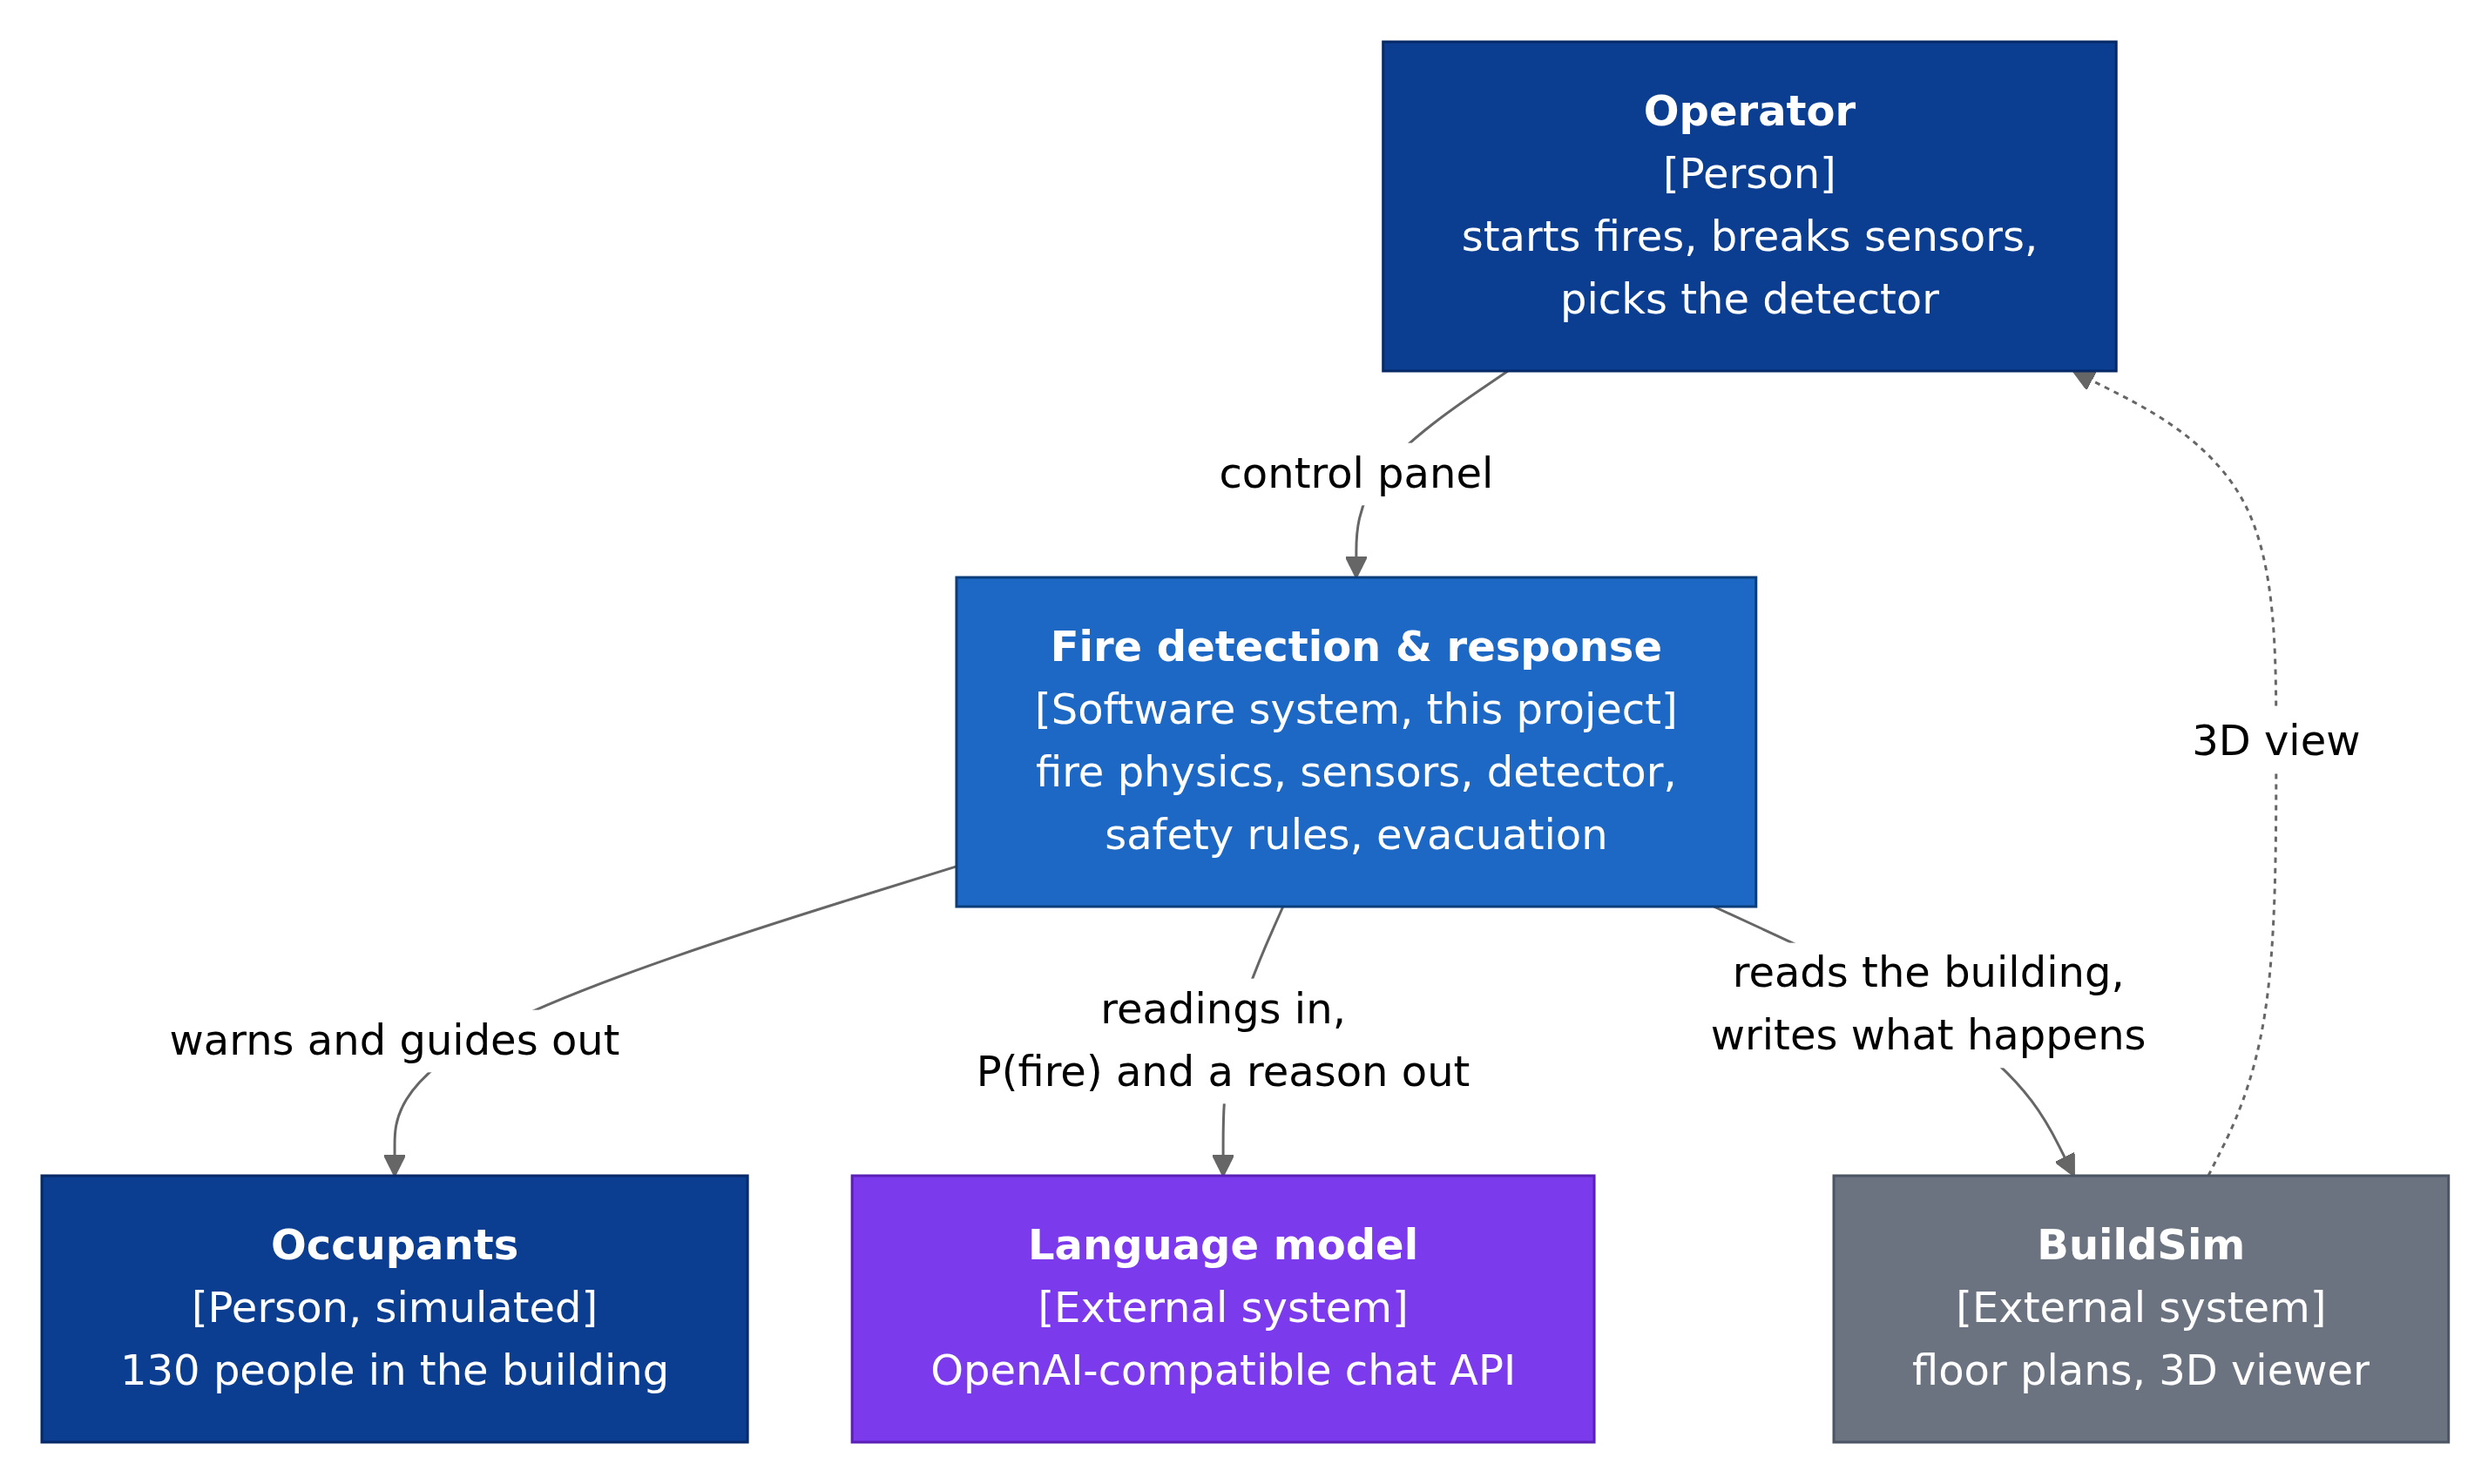
\includegraphics[width=0.78\linewidth]{images/context.png}
\caption{C4 System Context (Level 1). The system in scope is blue. BuildSim (grey) and the language model (purple) are outside it. Every arrow says what it carries. The model only ever gets readings, never the truth.}
\label{fig:context}
\end{figure}

\subsection{Container diagram (C4 Level 2)}\label{sec:container}

The container view opens the box. Five parts run separately, and two of them are my
code: the control panel in the browser and the firelab service. BuildSim and its 3D
viewer are provided. The fifth, the model endpoint, is the only one not on the
laptop. It is also the only one the system runs fine without.

\begin{figure}[H]
\centering
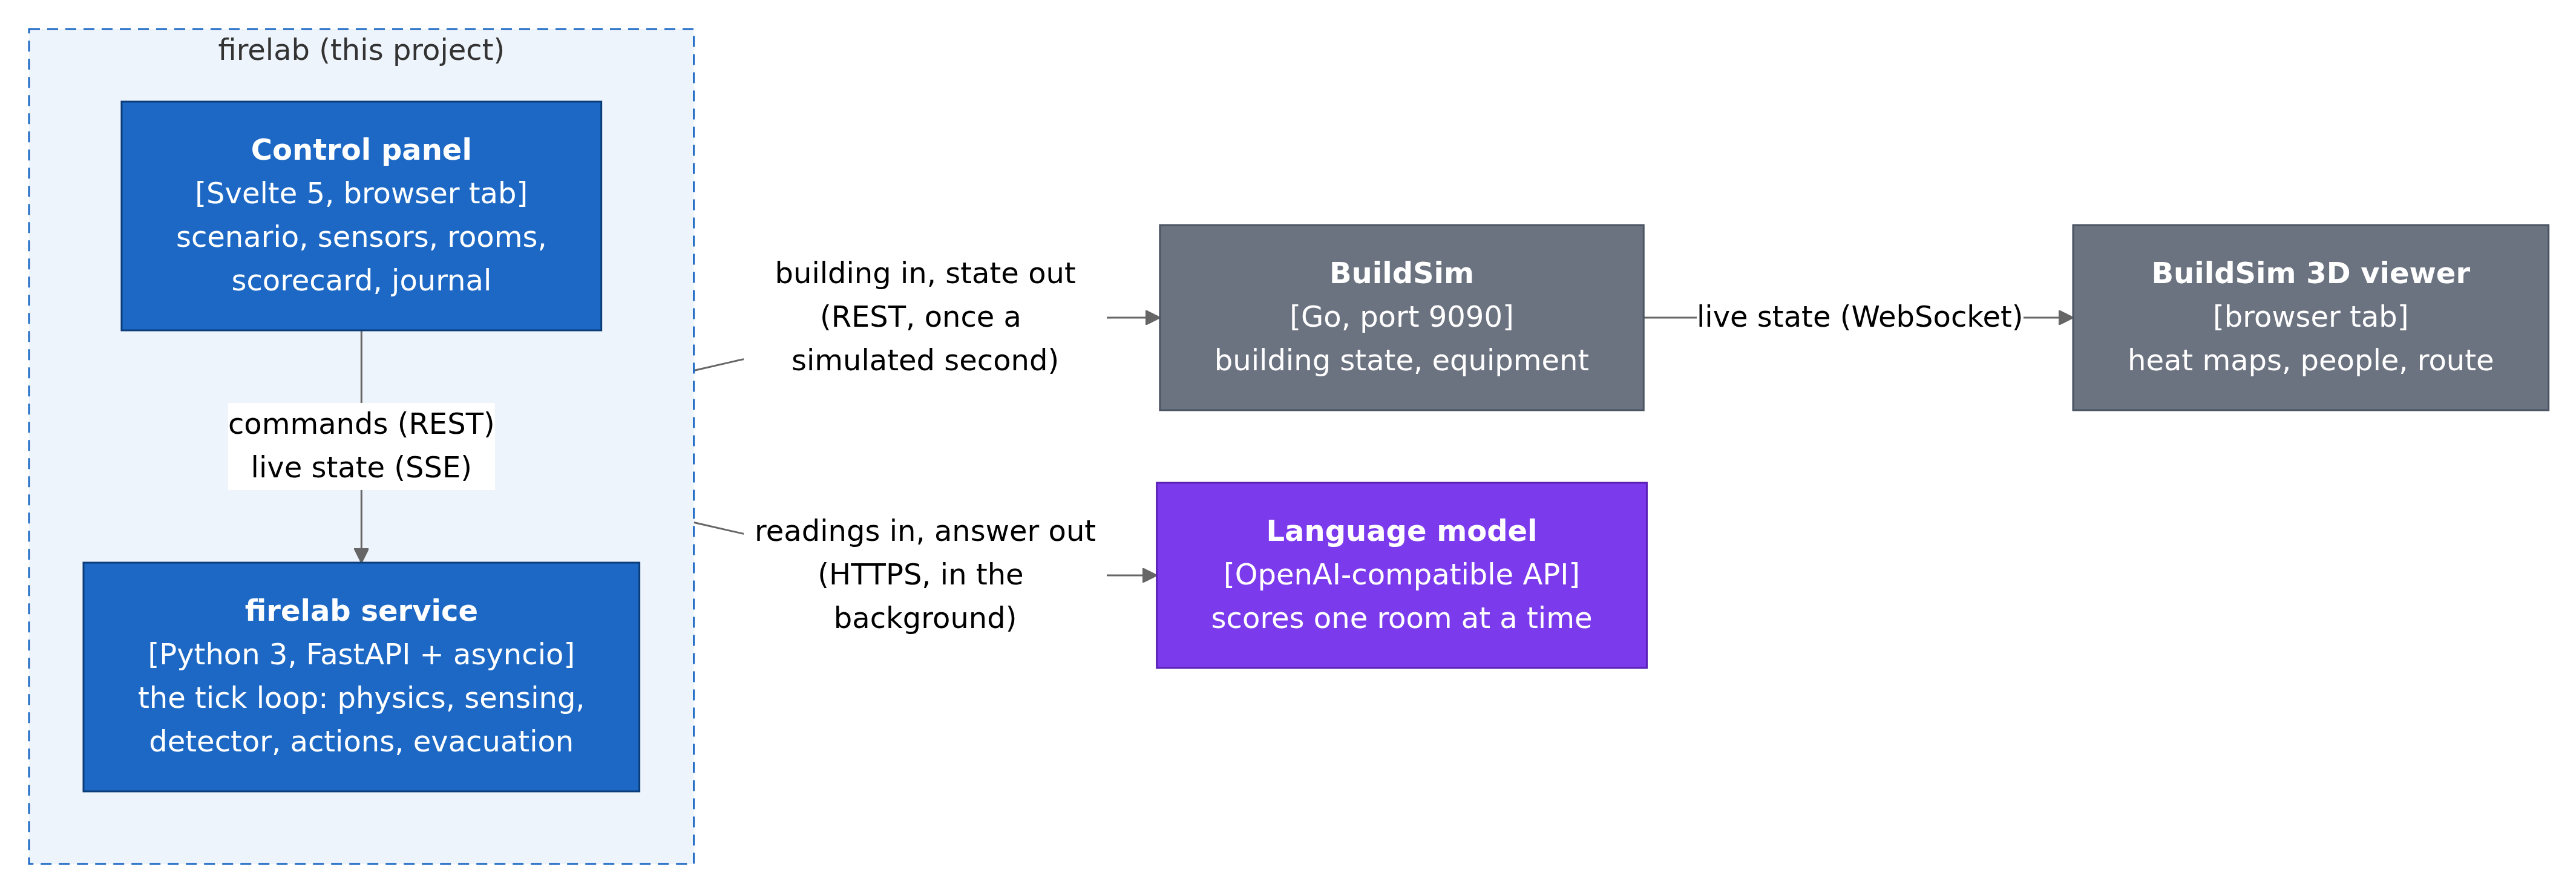
\includegraphics[width=0.90\linewidth]{images/container.png}
\caption{C4 Container diagram (Level 2). The dashed boundary is the system. BuildSim and its viewer are grey, and the language model is purple. Every arrow shows its protocol. A background task calls the model, never the tick.}
\label{fig:container}
\end{figure}

\textbf{Why one service.} In the proposal, nine containers would each have held one
of the four zones. I did not build it that way, for one reason: simulated time. The
whole point of the system is to run a fire at forty times real time. A 25-second
waiting time must still mean 25 simulated seconds. With a broker, every message
would need a simulated timestamp. Every subscriber would have to wait for every
publisher before moving on. A slow dashboard could stall the physics. Inside one
process, the tick loop does four things in a fixed order under one lock. It moves the
world forward, samples the sensors, thinks and acts. ``Now'' is one number. The
price is that the zones share a process, so a crash in one takes down the others.
Section~\ref{sec:risks} says what that costs and what would change if the system left the laptop.

\textbf{How one process does several things at once.} I built the service on
Python's \code{asyncio}. Think of it as one worker that juggles many small jobs.
Whenever a job has to wait, the worker puts it down and picks up another. Most of
the work here is waiting: for BuildSim to reply, for the model to reply, or for a
browser to collect the next update. Four jobs share the worker:
\begin{itemize}[nosep]
  \item the tick, which wakes every 250\,ms and moves the fire forward;
  \item the web API, which answers the control panel and streams live updates to
    each open browser tab;
  \item the publisher, which sends all its updates to BuildSim at once (six fixed
    ones plus one per sensor), so it only waits as long as the slowest one;
  \item the model's helper, which asks the language model its questions in the
    background.
\end{itemize}
I chose one worker instead of several threads because two jobs can then never
change the same data at the same moment. A job can only be paused at a point
where it waits. The tick also holds a lock while it runs, so a button press can
never change the building halfway through a tick. The downside is that a slow job
that never waits holds everyone up. That is why the tick must finish within
250\,ms, and why experiment E5 measures how many rooms fit in that time.

\textbf{What keeps the zones apart} is the package layering, since there are no
process boundaries. There are three packages. \code{domain} is pure: standard library
only, no clock, no network. \code{adapters} holds everything that speaks HTTP to
BuildSim. \code{app} holds the tick loop, the API and the snapshot. Dependencies only
point inward. A test, \code{test\_layering}, fails the build if any module imports
the wrong way. It also fails if anything in the intelligence path touches the true
room state.

\textbf{The control panel} is a separate container because it has a different
lifecycle. I build it once with Vite into static files, and the service serves them.
It talks to the service only through the REST endpoints and the server-sent event
stream. A script would use the same interface. The panel knows nothing about the
engine's internals.

\textbf{The model endpoint} is outside the boundary for the opposite reason. It is
not mine, and other users share it. It answers in about eight real seconds, while
the tick has 250 milliseconds. Those two facts shaped the adapter in front of it.
The service never waits for the model and asks it about one room at a time. It uses
an answer for at most a minute of simulated time. It also slows the clock to what the
measured answer time allows, so answers do not go stale (Section~\ref{sec:service}). I chose an
OpenAI-compatible chat API because every hosted and local model server speaks it.
So the endpoint, the key and the model name are three environment variables, and
nothing in the code names a vendor.

\subsection{Component diagram (C4 Level 3): inside the firelab service}\label{sec:component}

The service is the one container complex enough to need its own picture. Its
components are the four zones of one tick, plus the parts around them. The three
groups mark the truth boundary. Components in the orange group may read the real
state of the rooms. Components in the two blue groups may not. The only thing that
leaves the orange group is a sensor reading. I put the LLM adapter in the
readings-only group on purpose. It speaks HTTPS, so by the layering rules it lives
under \code{adapters}. But it sends the same feature vector the rule sees. The
layering test checks that it imports nothing that could tell it the truth.

\begin{figure}[H]
\centering
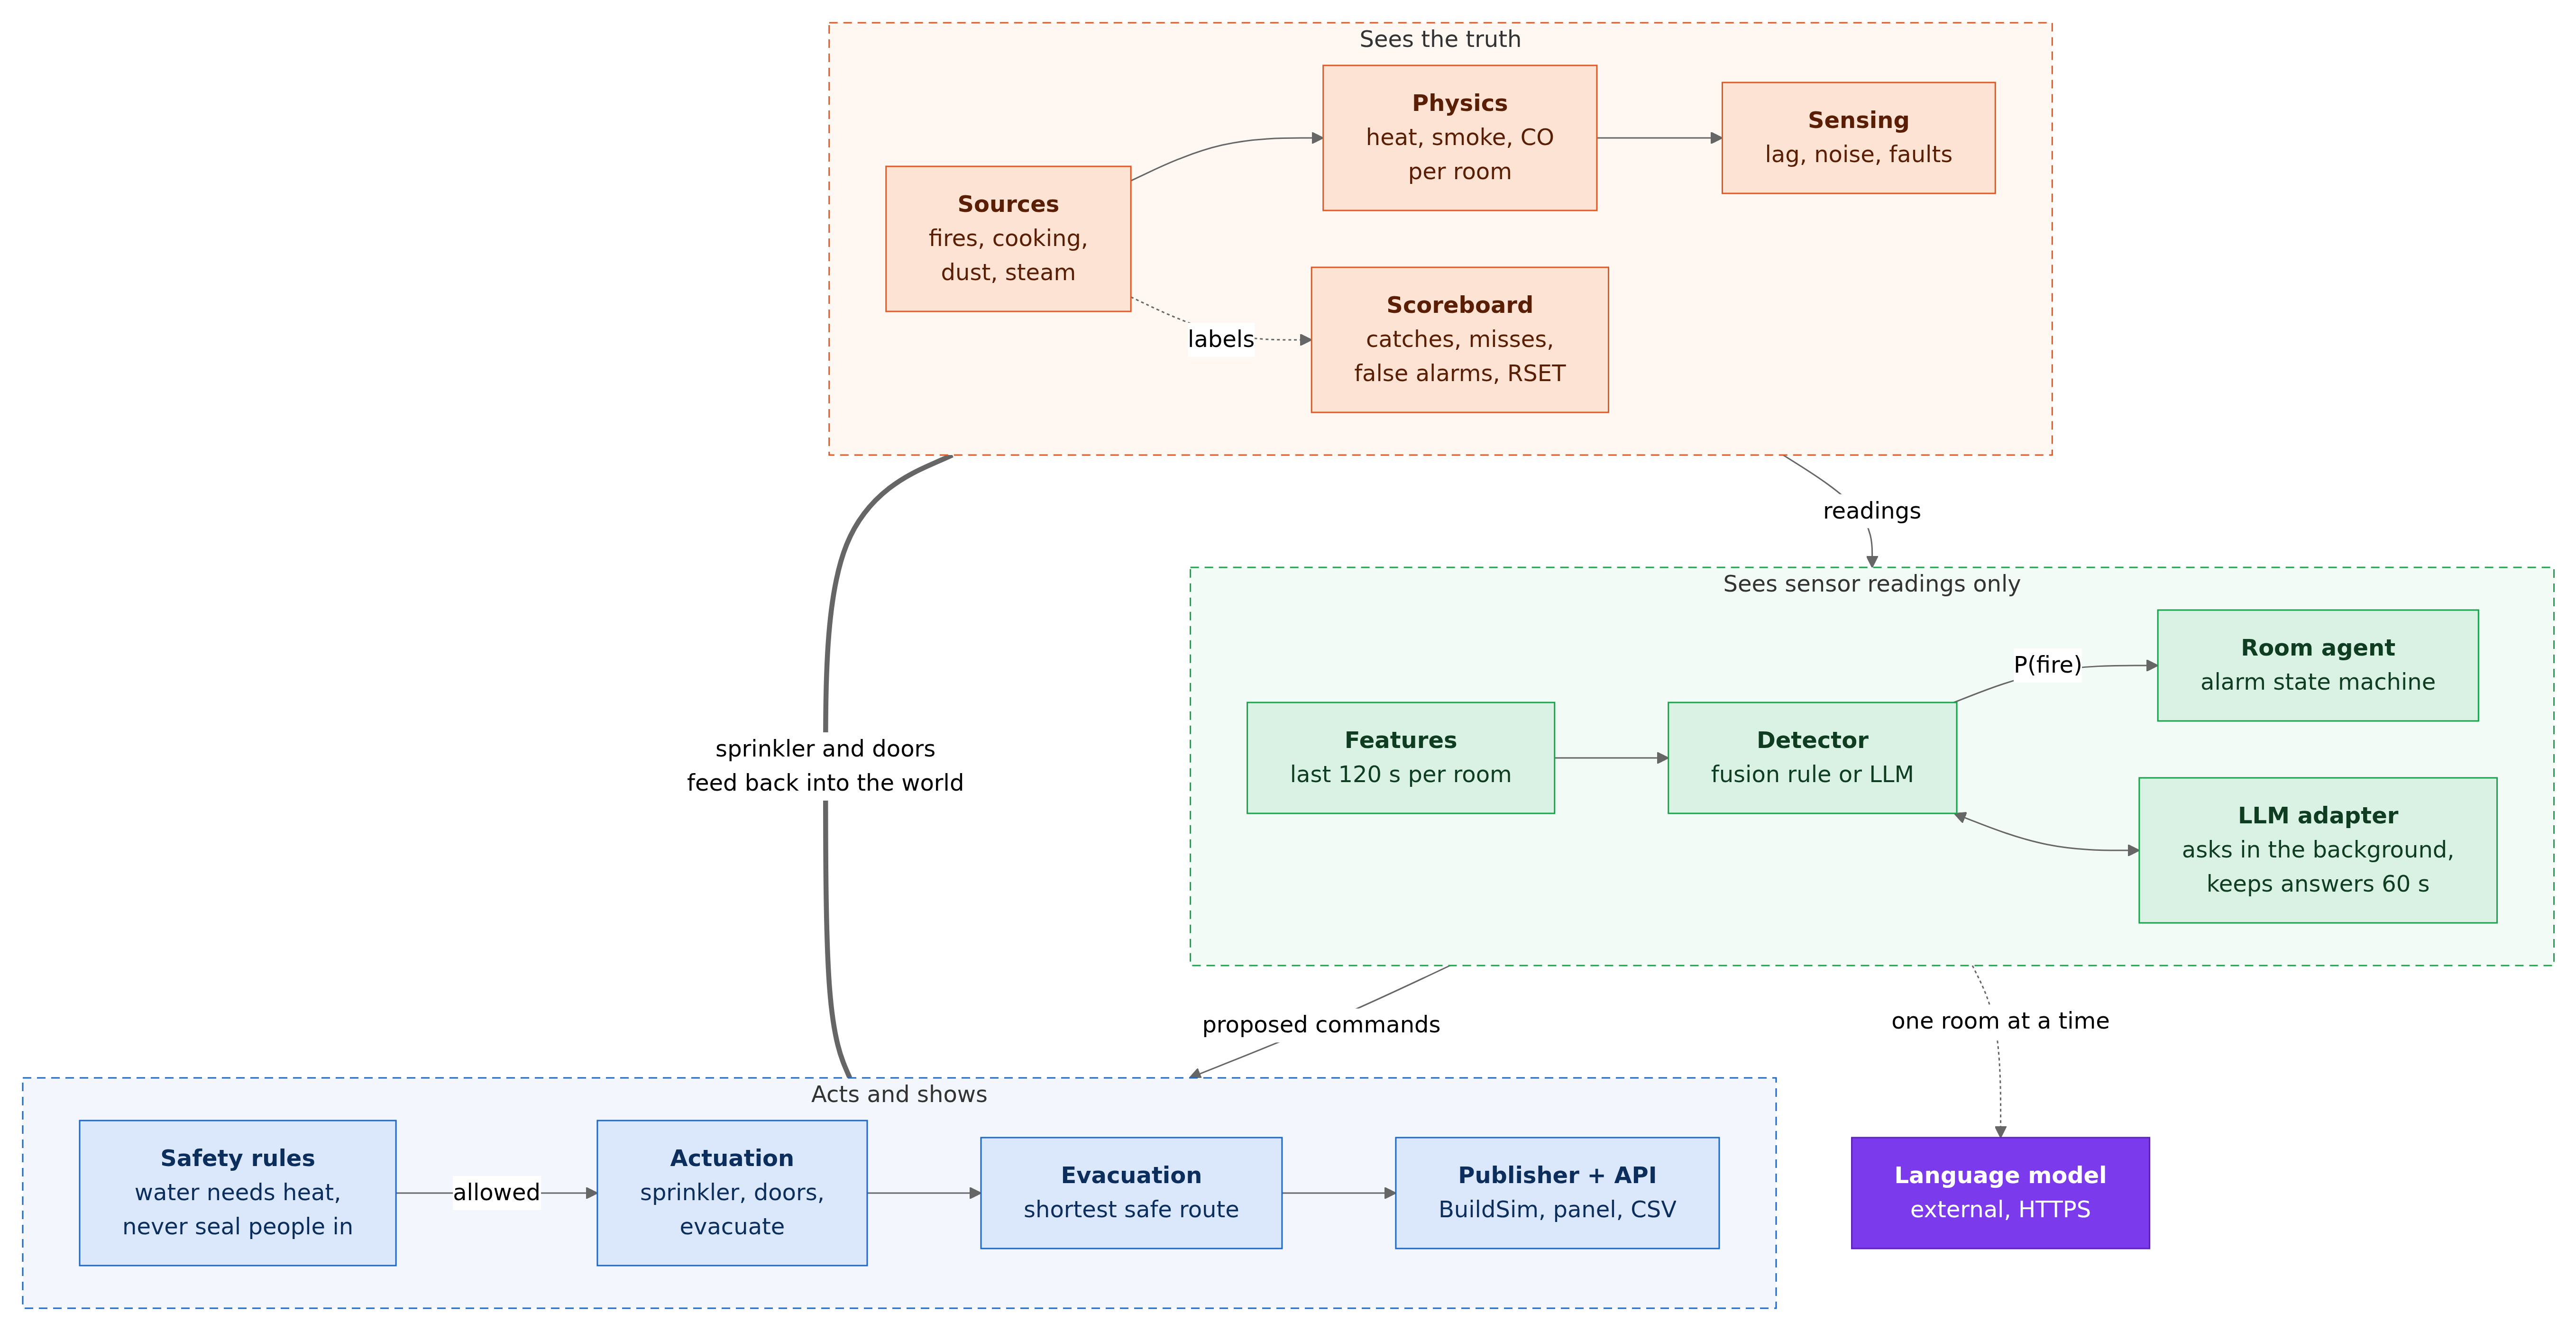
\includegraphics[width=1.00\linewidth]{images/component.png}
\caption{C4 Component diagram (Level 3) of the firelab service. The groups run in this order every tick: the orange group (the world and the sensors), then the green group (the detector and the agent), then the blue group (the actions). Only readings leave the orange group, and the layering test fails if anything else does. The thick line from the blue group back to the orange one is the sprinkler and door state being written into the world. The dotted arrow is the one call that leaves the process: the LLM adapter asking the language model about a room, outside the tick.}
\label{fig:component}
\end{figure}

\textbf{Component responsibilities.} Each component has one job. The last column
says why it is a separate component.

\begin{longtable}[]{@{}
  >{\raggedright\arraybackslash}p{(\columnwidth - 6\tabcolsep) * \real{0.15}}
  !{\colsep}>{\raggedright\arraybackslash}p{(\columnwidth - 6\tabcolsep) * \real{0.31}}
  !{\colsep}>{\raggedright\arraybackslash}p{(\columnwidth - 6\tabcolsep) * \real{0.24}}
  !{\colsep}>{\raggedright\arraybackslash}p{(\columnwidth - 6\tabcolsep) * \real{0.30}}@{}}
\toprule
\rowcolor{tablehead}
\textbf{Component} & \textbf{Responsibility (one job)} & \textbf{Module} & \textbf{Reason for separation} \\
\midrule
\endhead
Sources & What a fire, or cooking, dust or steam, gives off over time. Carries the ground-truth label & \code{domain/sources.py} & The label must never leak: only the scoreboard reads \code{kind} \\
\rowline
World / physics & One lumped node per room. Each node settles towards the level its sources drive it to, and spreads through doors and stairs & \code{domain/physics.py} & Owns every time constant, so each source stays a few lines long \\
\rowline
Sensing & Turns the truth into a reading through the corruption chain. Holds faults & \code{domain/sensing.py} & The line between truth and what is observed. The one place noise and faults live \\
\rowline
Features & A 120\,s window per room: rate of rise, ratio, neighbour agreement & \code{domain/features.py} & Sees readings only. This is the detector's input contract \\
\rowline
Detector & Turns features into P(fire), the estimated chance that the room is on fire, with a contribution per feature. The fusion rule (my hand-written rule that combines the sensor features into one score) is one implementation & \code{domain/detector.py} & A protocol, so a second detector can replace the rule without touching the agent. One did \\
\rowline
LLM adapter & The same protocol, answered from a cache of the model's answers. Asks in the background. The rule covers any room without a fresh answer & \code{adapters/llm/} & The network must never hold up the tick. One file per job (prompt, verdict, policy, client, detector), so each can be tested without an endpoint \\
\rowline
Room agent & The alarm ladder with waiting times. Proposes commands with reasons & \code{domain/agent.py} & Decides but never acts. Testable with no actuators \\
\rowline
Interlocks & Allows or refuses a command and says why & \code{domain/interlocks.py} & Kept outside the agent, so even a badly trained agent cannot trap anyone \\
\rowline
Actuation & The only door between deciding and doing. Writes sprinkler and door state into the world & \code{app/engine/actuation.py} & Closes the loop. One audit point for every change \\
\rowline
Evacuation & Routes people around danger, walks them, and picks the one route to draw & \code{app/evacuation.py}, \code{adapters/walkways.py} & The one domain-level job that needs a route lookup \\
\rowline
Scoreboard & Detections, misses, false alarms, RSET (the time people need to get out safely) and tenability (whether a room is still survivable) & \code{domain/scoring.py}, \code{timeline.py}, \code{tenability.py} & Grades the run. The only reader of the truth on the right-hand side \\
\rowline
Publisher + API & Turns engine state into BuildSim payloads and the UI snapshot. REST, SSE, CSV & \code{adapters/publisher/}, \code{app/api/}, \code{app/snapshot/} & Keeps presentation out of the loop. BuildSim's payload shapes live in one place \\
\bottomrule
\end{longtable}

\subsection{Design decisions and justifications}\label{sec:decisions}

Each row names the option I took, the alternative I considered, the requirement it
serves and the price paid. A decision with no rejected alternative would only be an
assumption.

\begin{longtable}[]{@{}
  >{\raggedright\arraybackslash}p{(\columnwidth - 8\tabcolsep) * \real{0.14}}
  !{\colsep}>{\raggedright\arraybackslash}p{(\columnwidth - 8\tabcolsep) * \real{0.20}}
  !{\colsep}>{\raggedright\arraybackslash}p{(\columnwidth - 8\tabcolsep) * \real{0.18}}
  !{\colsep}>{\raggedright\arraybackslash}p{(\columnwidth - 8\tabcolsep) * \real{0.30}}
  !{\colsep}>{\raggedright\arraybackslash}p{(\columnwidth - 8\tabcolsep) * \real{0.18}}@{}}
\toprule
\rowcolor{tablehead}
\textbf{Decision} & \textbf{Chosen} & \textbf{Alternatives} & \textbf{Justification (requirement)} & \textbf{Trade-off} \\
\midrule
\endhead
Process model & One tick loop, four zones, one lock & One container per zone over MQTT (the proposal) & Waiting times and rates need one simulated clock. At 40$\times$, a reading sent through a broker is stale when it arrives (NFR-01, NFR-03) & No fault isolation between zones. Splitting them is a future step \\
\rowline
Concurrency & \code{asyncio}: one worker that switches between jobs while they wait & Several threads; one process per job & The work is mostly waiting on the network. With one worker, two jobs never change the same data at once, and the tick's lock covers the rest (NFR-01, NFR-03) & A slow job that never waits holds everyone up, so the tick must finish within 250\,ms \\
\rowline
Zone separation & Import layering checked by a test & Trust the code review & The truth is one attribute away from the detector. A test lets me check that the code keeps away from it (NFR-04) & A test to maintain as modules move \\
\rowline
Detector & Hand-written fusion rule behind a protocol, as the default & Isolation forest; autoencoder; the model alone & It caught every fire, with zero false alarms at every noise level. It explains itself term by term and costs nothing per room (FR-01, FR-03, FR-06) & Weights tuned by hand. No learning from data \\
\rowline
Second detector & A language model over an OpenAI-compatible API, given readings only & Isolation forest trained on exported runs; no second detector & This is the comparison the proposal promised, without training on the simulator's own output. The answer comes with evidence and a reason, so FR-06 still holds (FR-08) & About 8\,s per answer, not repeatable, and an outside dependency \\
\rowline
Model off the tick & Background worker, cached answers good for 60\,s, rule fallback & Ask and wait for the reply; use stale answers & A tick has 250\,ms and an answer takes seconds. A room must always have a number, and a stale number is a wrong one (NFR-06, NFR-07) & Two detectors are in play at once, and the journal has to say which one is speaking \\
\rowline
Pacing & Cap the speed dial at what measured answer times allow & Let the clock run and accept that answers expire & At 40$\times$, every answer arrived 320 simulated seconds late, and the rule quietly did all the work. A capped dial is honest (NFR-07) & With this endpoint, the demo runs at 3$\times$ instead of 40$\times$ \\
\rowline
Questions in flight & One at a time, most suspicious room first & Several at once & The endpoint answers requests one after another. Two in flight doubled the delay and halved the speed the clock could run at. The fire room gets its answer first & The rule scores most of the quiet neighbours \\
\rowline
Alarm logic & State machine with waiting times & Threshold on P(fire) & A single threshold flickers with noise. Waiting times cost seconds, but they stop doors opening and closing over and over (FR-03) & Adds 45\,s to confirming a clear fire \\
\rowline
Safety & Safety rules outside the agent & Rules inside the agent's policy & Whoever is wrong upstream, the building stays safe. The same check applies to a person's click (SR-01 to SR-03) & A confirmed fire in an occupied room gets no door \\
\rowline
Deferred commands & A refused request stands until it can be carried out & Refuse once and forget & ``Not yet'' must not become ``never''. In the smoulder, the sprinkler was refused at 201\,s and released at 219\,s, once heat arrived (SR-01) & Re-checked every tick \\
\rowline
Route search & My own Dijkstra search over BuildSim's graph, with alarming rooms removed & Ask BuildSim's router for each exit & BuildSim only returns the shortest path. A fire in a corridor makes every shortest path run through it (FR-05) & A second copy of the graph to keep consistent \\
\rowline
Sensor emulation & Lag, bias, noise, quantisation, clamp, faults per device & Truth plus Gaussian noise & The interesting failures (saturation, stuck, dead) are not noise. The temperature clamp at 250\,°C is what a real heat detector does (NFR-02) & More parameters to defend \\
\rowline
Physics & Lumped node per room, first-order relaxation, door-gated diffusion & CFD; zone model with layers & Enough structure to close the loop and get the trends right. Cheap enough for 956 rooms 40 times a second (NFR-01) & The fire room overheats when sealed. No oxygen limit (Section~\ref{sec:risks}) \\
\rowline
Storage & In-memory rolling windows; CSV export & Time-series database; ThingsBoard & The detector may only see 120\,s, and the charts only need 20 minutes. A database would be one more process to keep in step with the clock (NFR-01) & History is lost on restart. Long runs are exported, not stored \\
\rowline
UI transport & Server-sent events, one snapshot per tick & Polling; WebSocket & One-way push with automatic reconnect, and a plain HTTP stream any tool can read & The snapshot is rebuilt every tick, even with no listener \\
\rowline
BuildSim writes & Once per simulated second, complete collections, 24 sensor values per publish & Every tick; deltas & BuildSim replaces a whole collection on each write. Too many writes overloaded it (NFR-05) & Sensor labels in the tree lag behind the truth \\
\bottomrule
\end{longtable}

\section{Interfaces and communication}\label{sec:interfaces}

I use four patterns, each where it fits. \textbf{REST} carries every command and
every call to BuildSim. Each is a one-to-one request, and the caller must know the
result. For example, a refused command comes back with the safety rule's reason.
\textbf{Server-sent events} carry the snapshot to the control panel. That flow is
one-way and high-rate, and it needs no reply. \textbf{WebSocket} is BuildSim's own
channel to its viewer. I use it, but I did not build it. \textbf{HTTPS chat
completions} carry one room's readings to the language model and a JSON answer back.
A background task makes the call, with a 30\,s timeout and one retry. The result
goes into a cache, never into a tick. There is no pub/sub, for the reason given in
Section~\ref{sec:container}.

\textbf{Naming.} Everywhere, a room's address is \code{level/name}, for instance
\code{level2/A3505}. I do this because a bare name is not unique across storeys. A
device is \code{fl-<level>-<room>-<modality>}, so you can read its room and sensor
type off its ID. Units are fixed and never sent in messages: temperature in °C,
smoke as optical obscuration in 1/m, CO in ppm, distances on the plan in half-metre
units, and simulated time in seconds since midnight.

\textbf{The control-panel API.} Every request body is a typed model. The framework
rejects unknown keys before the engine sees them.

\begin{longtable}[]{@{}
  >{\raggedright\arraybackslash}p{(\columnwidth - 6\tabcolsep) * \real{0.10}}
  !{\colsep}>{\raggedright\arraybackslash}p{(\columnwidth - 6\tabcolsep) * \real{0.30}}
  !{\colsep}>{\raggedright\arraybackslash}p{(\columnwidth - 6\tabcolsep) * \real{0.30}}
  !{\colsep}>{\raggedright\arraybackslash}p{(\columnwidth - 6\tabcolsep) * \real{0.30}}@{}}
\toprule
\rowcolor{tablehead}
\textbf{Method} & \textbf{Path} & \textbf{Body} & \textbf{Semantics} \\
\midrule
\endhead
GET & \code{/api/state} & & The full snapshot, once \\
\rowline
GET & \code{/api/events} & & SSE: one snapshot per tick, 4\,Hz \\
\rowline
GET & \code{/api/rooms} & & Every space for the pickers \\
\rowline
GET, PUT & \code{/api/config} & partial config & Live settings: speed, thresholds, waiting times, noise, population. \code{detector.kind} swaps the detector on the next tick \\
\rowline
POST & \code{/api/clock} & \code{\{seconds?, factor?, running?\}} & Play, pause, jump, 0.1--600$\times$ \\
\rowline
POST & \code{/api/scenario/ignite} & \code{\{space, kind, growth, delay, peak\_kw\}} & Schedule a source. \code{kind} is also the label \\
\rowline
POST & \code{/api/scenario/preset} & \code{\{preset, space\}} & Put sensors in the room and its neighbours, then ignite \\
\rowline
DELETE & \code{/api/scenario/\{id\}} & & Put a source out. What it gave off still spreads \\
\rowline
POST & \code{/api/sensors/deploy} & \code{\{spaces, modalities\}} & Install devices. A room without devices is not monitored \\
\rowline
POST & \code{/api/sensors/fault} & \code{\{device\_id, fault\}} & \code{stuck | dropout | drift | dead | none} \\
\rowline
POST & \code{/api/agent/mode} & \code{\{auto\}} & \code{false} means supervised: decisions are shown, not carried out \\
\rowline
POST & \code{/api/actuators/command} & \code{\{kind, space, value\}} & A manual command. It passes the same safety rules and returns \code{\{allowed, reason\}} \\
\rowline
GET & \code{/api/history?space=} & & The last 240 samples of one room \\
\rowline
GET & \code{/api/export.csv} & & Truth beside reading beside P(fire), every room, labelled \\
\rowline
POST & \code{/api/reset}, \code{/api/reload} & & Quiet building. Reload floors from BuildSim \\
\bottomrule
\end{longtable}

\textbf{The snapshot} is the one data structure the panel reads. Each monitored room
appears as shown below. The three columns of the Rooms table are the three objects
in it: what is true, what was reported, and what the system believes.

\begin{verbatim}
{"key": "level2/A3505", "level": "level2", "name": "A3505", "kind": "room",
 "truth":   {"temperature": 648.0, "smoke": 0.668, "co": 107.0},
 "reading": {"temperature": 250.0, "smoke": 0.665, "co": 101.0},
 "p_fire": 0.994, "state": "CONFIRMED", "tenable": false,
 "sprinkler": true, "door": "closed", "occupants": 0,
 "devices": [{"id": "fl-level2-A3505-smoke", "modality": "smoke",
              "fault": "none", "reading": 0.665}, ...]}
\end{verbatim}

The temperature reading of 250 against a truth of 648 is not a bug in the example.
It is the heat detector's range clamp. The snapshot exists to make this kind of
thing visible.

\textbf{The BuildSim interface.} I publish truth and belief to different endpoints.
So a false positive shows on screen as a room glowing red on the belief layer while
it is cool on the heat map.

\begin{longtable}[]{@{}
  >{\raggedright\arraybackslash}p{(\columnwidth - 6\tabcolsep) * \real{0.36}}
  !{\colsep}>{\raggedright\arraybackslash}p{(\columnwidth - 6\tabcolsep) * \real{0.10}}
  !{\colsep}>{\raggedright\arraybackslash}p{(\columnwidth - 6\tabcolsep) * \real{0.32}}
  !{\colsep}>{\raggedright\arraybackslash}p{(\columnwidth - 6\tabcolsep) * \real{0.22}}@{}}
\toprule
\rowcolor{tablehead}
\textbf{Endpoint} & \textbf{Direction} & \textbf{Carries} & \textbf{When} \\
\midrule
\endhead
\code{GET /api/building/floors/\{level\}} & read & rooms, polygons, walkable graph & once, at load \\
\rowline
\code{GET /api/building/cross-floor-edges} & read & stairs and lifts joining storeys & once, at load \\
\rowline
\code{GET /api/graph/route} & read & a shortest path, multi-floor & fallback when no clear route exists \\
\rowline
\code{PUT /api/room-layers} & write & true temperature, smoke, CO; and P(fire) as its own layer & every simulated second \\
\rowline
\code{PUT /api/effects} & write & fire, smoke and sprinkler particles & every simulated second \\
\rowline
\code{PUT /api/alerts} & write & the agent's alarm markers with P(fire) & every simulated second \\
\rowline
\code{PUT /api/doors} & write & fire-door state. Also blocks the walkable router & every simulated second \\
\rowline
\code{PUT /api/entities}, \code{/api/occupancy} & write & every occupant's position and figure; head count per room & every simulated second \\
\rowline
\code{PUT /api/sensors/\{id\}/value} & write & one device's latest reading, into the equipment tree & 24 per publish, round robin \\
\rowline
\code{PUT /api/sessions/\{id\}/highlights} & write & red, orange, yellow outlines by alarm state & when they change \\
\rowline
\code{PUT /api/sessions/\{id\}/route} & write & the one escape route drawn, each node with its storey & when it changes \\
\bottomrule
\end{longtable}

A route is a list of waypoints plus its length in metres. Each waypoint carries its
level, so a path down the stairs is drawn on each storey it crosses. A closed door
goes to BuildSim as well as into the physics. That way BuildSim's own router, which
the viewer's route finder uses, stops sending people into a sealed room.

\textbf{The model interface.} There is one request per room:
\code{POST /chat/completions} on whatever base URL is configured. It holds the fixed
system prompt and the room's readings as plain lines with units. The prompt is the
whole contract. It tells the model that it sees only the sensors, never the room. It
also lists what separates a fire from cooking, dust or steam, in the same terms the
rule uses. The reply must be one JSON object:

\begin{verbatim}
{"p_fire": 0.92,
 "evidence": [{"name": "CO 95 ppm", "weight": 0.30},
              {"name": "smoke rising", "weight": 0.25}, ...],
 "reason": "Smoke, CO and temperature are rising together."}
\end{verbatim}

The service refuses any reply that does not parse as that, or whose probability is
not a number. It does not try to repair it, and the room stays with the rule. The
evidence becomes the ``Why'' bars on the panel. Next to them is a bar for the answer
itself, on the rule's logit scale. That way the two detectors read the same way on
screen.
